\section{Basic}
\subsection{vimrc}
\lstinputlisting{01_Basic/.vimrc}
\subsection{Default code}
\lstinputlisting{01_Basic/default_code.cpp}
\subsection{readchar}
\lstinputlisting{01_Basic/readchar.cpp}
\subsection{readint}
\lstinputlisting{01_Basic/readint.cpp}
\subsection{Black Magic}
\lstinputlisting{01_Basic/black_magic.cpp}

\section{Graph}
\subsection{BCC Vertex*} % test by CF 102512 A
\lstinputlisting{02_Graph/BCC_Vertex.cpp}
\subsection{Bridge*} % test by TIOJ 1879
\lstinputlisting{02_Graph/Bridge.cpp}
\subsection{Bipartite Matching*} % test by TIOJ 1879
\lstinputlisting{02_Graph/Bipartite_Matching.cpp}
\subsection{2SAT (SCC)*} % SCC test by TIOJ 2143, 2SAT test by ARC069 F
\lstinputlisting{02_Graph/2SAT.cpp}
\subsection{MinimumMeanCycle*} % test by TIOJ 1934
\lstinputlisting{02_Graph/MinimumMeanCycle.cpp}
\subsection{Maximum Clique Dyn*} % test by TIOJ 1978
\lstinputlisting{02_Graph/Maximum_Clique_Dyn.cpp} 
\subsection{Maximum Clique*} % test by TIOJ 1978
\lstinputlisting{02_Graph/Maximum_Clique.cpp}
\subsection{Minimum Steiner Tree*} % test by luogu P6192
\lstinputlisting{02_Graph/MinimumSteinerTree.cpp}
\subsection{Minimum Arborescence*} % test by NTUJ 2176
\lstinputlisting{02_Graph/Minimum_Arborescence.cpp}
\subsection{Vizing's theorem}
\lstinputlisting{02_Graph/Vizing.cpp}
\subsection{Minimum Clique Cover*} % test by TIOJ 1472
\lstinputlisting{02_Graph/Minimum_Clique_Cover.cpp}
\subsection{NumberofMaximalClique*} % test by POJ 2989
\lstinputlisting{02_Graph/NumberofMaximalClique.cpp}
\subsection{Dijkstra*}
\lstinputlisting{02_Graph/Dijkstra.cpp}
\subsection{Kosaraju*}
\lstinputlisting{02_Graph/Kosaraju.cpp}
\subsection{Simple Graph Matching*}
\lstinputlisting{02_Graph/Simple_Graph_Matching.cpp}
\subsection{Two Edge Connected Components}
\lstinputlisting{02_Graph/Two_Edge_connected_components.cpp}
\subsection{Theory}
\begin{footnotesize}
$|$Maximum independent edge set$|=|V|-|$Minimum edge cover$|$\\
$|$Maximum independent set$|=|V|-|$Minimum vertex cover$|$\\
\end{footnotesize}
\subsection{LCA*}
\lstinputlisting{02_Graph/LCA.cpp}
\subsection{Tree Flatten*}
\lstinputlisting{02_Graph/Tree_Flatten.cpp}


\section{Data Structure}
\subsection{Leftist Tree}
\lstinputlisting{03_Data_Structure/Leftist_Tree.cpp}
\subsection{Heavy light Decomposition}
\lstinputlisting{03_Data_Structure/Heavy_light_Decomposition.cpp}
\subsection{Centroid Decomposition*} % test by TIOJ 1171
\lstinputlisting{03_Data_Structure/Centroid_Decomposition.cpp}
\subsection{Smart Pointer*}
\lstinputlisting{03_Data_Structure/Smart_Pointer.cpp}
\subsection{LiChaoST*}
\lstinputlisting{03_Data_Structure/LiChaoST.cpp}
\subsection{LiChaoSTSeg*}
\lstinputlisting{03_Data_Structure/LiChaoSTSeg.cpp}
\subsection{Link cut tree*} % test by luogu P3690
\lstinputlisting{03_Data_Structure/link_cut_tree.cpp}
\subsection{KDTree}
\lstinputlisting{03_Data_Structure/KDTree.cpp}
\subsection{Segment Tree with tag}
\lstinputlisting{03_Data_Structure/Segment_Tree_with_tag.cpp}
\subsection{2D Binary Indexed Tree}
\lstinputlisting{03_Data_Structure/2D_Binary_Indexed_Tree.cpp}


\section{Flow/Matching}
\subsection{Dinic}
\lstinputlisting{04_Flow_Matching/Dinic.cpp}
% \subsection{Kuhn Munkres}
% \lstinputlisting{04_Flow_Matching/Kuhn_Munkres.cpp}
% \subsection{MincostMaxflow}
% \lstinputlisting{04_Flow_Matching/MincostMaxflow.cpp}
% \subsection{Maximum Simple Graph Matching*} % test by TIOJ 1504
% \lstinputlisting{04_Flow_Matching/Maximum_Simple_Graph_Matching.cpp}
% \subsection{Minimum Weight Matching (Clique version)*} % test by uoj.ac 81
% \lstinputlisting{04_Flow_Matching/Minimum_Weight_Matching.cpp}
% \subsection{SW-mincut}
% \lstinputlisting{04_Flow_Matching/SW-mincut.cpp}
% \subsection{BoundedFlow(Dinic*)} % test by NTUJ 184(Only Dinic)
% \lstinputlisting{04_Flow_Matching/BoundedFlow.cpp}
% \subsection{Flow Models}
% % \normalsize
\begin{itemize}
    \itemsep-0.3em
    \item Maximum/Minimum flow with lower bound / Circulation problem
    \vspace{-1em}
    \begin{enumerate}
        \itemsep-0.3em
        \item Construct super source $S$ and sink $T$.
        \item For each edge $(x, y, l, u)$, connect $x \rightarrow y$ with capacity $u - l$.
        \item For each vertex $v$, denote by $in(v)$ the difference between the sum of incoming lower bounds and the sum of outgoing lower bounds.
        \item If $in(v) > 0$, connect $S \rightarrow v$ with capacity $in(v)$, otherwise, connect $v \rightarrow T$ with capacity $-in(v)$.
        \begin{itemize}
            \itemsep-0.2em
            \item To maximize, connect $t \rightarrow s$ with capacity $\infty$ (skip this in circulation problem), and let $f$ be the maximum flow from $S$ to $T$. If $f \neq \sum_{v \in V, in(v) > 0}{in(v)}$, there's no solution. Otherwise, the maximum flow from $s$ to $t$ is the answer.
            \item To minimize, let $f$ be the maximum flow from $S$ to $T$. Connect $t \rightarrow s$ with capacity $\infty$ and let the flow from $S$ to $T$ be $f^\prime$. If $f + f^\prime \neq \sum_{v \in V, in(v) > 0}{in(v)}$, there's no solution. Otherwise, $f^\prime$ is the answer.
        \end{itemize}
        \item The solution of each edge $e$ is $l_e + f_e$, where $f_e$ corresponds to the flow of edge $e$ on the graph.
    \end{enumerate}
    \item Construct minimum vertex cover from maximum matching $M$ on bipartite graph $(X, Y)$
    \vspace{-1em}
    \begin{enumerate}
        \itemsep-0.3em
        \item Redirect every edge: $y \rightarrow x$ if $(x, y) \in M$, $x \rightarrow y$ otherwise.
        \item DFS from unmatched vertices in $X$.
        \item $x \in X$ is chosen iff $x$ is unvisited.
        \item $y \in Y$ is chosen iff $y$ is visited.
    \end{enumerate}
    \item Minimum cost cyclic flow
    \vspace{-0.5em}
    \begin{enumerate}
        \itemsep-0.3em
        \item Consruct super source $S$ and sink $T$
        \item For each edge $(x, y, c)$, connect $x \rightarrow y$ with $(cost, cap) = (c, 1)$ if $c > 0$, otherwise connect $y \rightarrow x$ with $(cost, cap) = (-c, 1)$
        \item For each edge with $c < 0$, sum these cost as $K$, then increase $d(y)$ by 1, decrease $d(x)$ by 1
        \item For each vertex $v$ with $d(v) > 0$, connect $S \rightarrow v$ with $(cost, cap) = (0, d(v))$
        \item For each vertex $v$ with $d(v) < 0$, connect $v \rightarrow T$ with $(cost, cap) = (0, -d(v))$
        \item Flow from $S$ to $T$, the answer is the cost of the flow $C + K$
    \end{enumerate}
    \item Maximum density induced subgraph
    \vspace{-1em}
    \begin{enumerate}
        \itemsep-0.3em
        \item Binary search on answer, suppose we're checking answer $T$
        \item Construct a max flow model, let $K$ be the sum of all weights
        \item Connect source $s \rightarrow v$, $v \in G$ with capacity $K$
        \item For each edge $(u, v, w)$ in $G$, connect $u \rightarrow v$ and $v \rightarrow u$ with capacity $w$
        \item For $v \in G$, connect it with sink $v \rightarrow t$ with capacity $K + 2T - (\sum_{e \in E(v)}{w(e)}) - 2w(v)$
        \item $T$ is a valid answer if the maximum flow $f < K \lvert V \rvert$
    \end{enumerate}
    \item Minimum weight edge cover
    \vspace{-1em}
    \begin{enumerate}
        \itemsep-0.3em
      \item For each $v \in V$ create a copy $v^\prime$, and connect $u^\prime \to v^\prime$ with weight $w(u, v)$.
      \item Connect $v \to v^\prime$ with weight $2\mu(v)$, where $\mu(v)$ is the cost of the cheapest edge incident to $v$.
      \item Find the minimum weight perfect matching on $G^\prime$.
    \end{enumerate}
    \item Project selection problem
    \vspace{-1em}
    \begin{enumerate}
      \itemsep-0.3em
      \item If $p_v > 0$, create edge $(s, v)$ with capacity $p_v$; otherwise, create edge $(v, t)$ with capacity $-p_v$.
      \item Create edge $(u, v)$ with capacity $w$ with $w$ being the cost of choosing $u$ without choosing $v$.
      \item The mincut is equivalent to the maximum profit of a subset of projects.
    \end{enumerate}
    \item 0/1 quadratic programming
    \vspace{-1em}
    \[ \sum_x{c_xx} + \sum_y{c_y\bar{y}} + \sum_{xy}c_{xy}x\bar{y} + \sum_{xyx^\prime y^\prime}c_{xyx^\prime y^\prime}(x\bar{y} + x^\prime\bar{y^\prime}) \]
    can be minimized by the mincut of the following graph:
    \begin{enumerate}
      \itemsep-0.3em
      \item Create edge $(x, t)$ with capacity $c_x$ and create edge $(s, y)$ with capacity $c_y$.
      \item Create edge $(x, y)$ with capacity $c_{xy}$.
      \item Create edge $(x, y)$ and edge $(x^\prime, y^\prime)$ with capacity $c_{xyx^\prime y^\prime}$.
    \end{enumerate}
\end{itemize}

% \subsection{isap}
% \lstinputlisting{04_Flow_Matching/isap.cpp}


\section{String}
\subsection{KMP}
\lstinputlisting{05_String/KMP.cpp}
\subsection{Z-value}
\lstinputlisting{05_String/Z-value.cpp}
\subsection{Manacher*} % test by TIOJ 1276
\lstinputlisting{05_String/Manacher.cpp}
\subsection{SAIS*}
\lstinputlisting{05_String/SAIS.cpp}
\subsection{Aho-Corasick Automaton}
\lstinputlisting{05_String/Aho-Corasick_Automaton.cpp}
\subsection{Smallest Rotation}
\lstinputlisting{05_String/Smallest_Rotation.cpp}
\subsection{De Bruijn sequence*} % test by CF 102001 C
\lstinputlisting{05_String/De_Bruijn_sequence.cpp}
\subsection{SAM}
\lstinputlisting{05_String/SAM.cpp}
\subsection{PalTree}
\lstinputlisting{05_String/PalTree.cpp}
\subsection{cyclicLCS}
\lstinputlisting{05_String/cyclicLCS.cpp}
\subsection{Suffix Array}
\lstinputlisting{05_String/Suffix_Array.cpp}
\subsection{Suffix Array2}
\lstinputlisting{05_String/Suffix_Array2.cpp}


\section{Math}
\subsection{exgcd*} % test by NTUJ 110
\lstinputlisting{06_Math/exgcd.cpp}
\subsection{floor and ceil}
\lstinputlisting{06_Math/floor_ceil.cpp}
\subsection{SG value}
\lstinputlisting{06_Math/SG_value.cpp}
% \subsection{floor sum*} % test by AtCoder Library Practice Contest C, CF 100920 J
% \lstinputlisting{06_Math/floor_sum.cpp}
\subsection{Miller Rabin*} % test by NTUJ 1237
\lstinputlisting{06_Math/Miller_Rabin.cpp}
\subsection{Big number}
\lstinputlisting{06_Math/Big_number.cpp}
\subsection{Fraction}
\lstinputlisting{06_Math/Fraction.cpp}
\subsection{Simultaneous Equations}
\lstinputlisting{06_Math/Simultaneous_Equations.cpp}
\subsection{Pollard Rho}
\lstinputlisting{06_Math/Pollard_Rho.cpp}
\subsection{Simplex Algorithm}
\lstinputlisting{06_Math/Simplex_Algorithm.cpp}
\subsubsection{Construction}
% \normalsize
Standard form: maximize $\mathbf{c}^T\mathbf{x}$ subject to $A\mathbf{x} \leq \mathbf{b}$ and $\mathbf{x} \geq 0$. \\
Dual LP: minimize $\mathbf{b}^T\mathbf{y}$ subject to $A^T\mathbf{y} \geq \mathbf{c}$ and $\mathbf{y} \geq 0$. \\
$\bar{\mathbf{x}}$ and $\bar{\mathbf{y}}$ are optimal if and only if for all $i \in [1, n]$, either $\bar{x}_i = 0$ or $\sum_{j=1}^{m}A_{ji}\bar{y}_j = c_i$ holds and for all $i \in [1, m]$ either $\bar{y}_i = 0$ or $\sum_{j=1}^{n}A_{ij}\bar{x}_j = b_j$ holds.

\begin{enumerate}
    \itemsep-0.5em
    \item In case of minimization, let $c^\prime_i = -c_i$
    \item $\sum_{1 \leq i \leq n}{A_{ji}x_i} \geq b_j \rightarrow \sum_{1 \leq i \leq n}{-A_{ji}x_i} \leq -b_j$
    \item $\sum_{1 \leq i \leq n}{A_{ji}x_i} = b_j$ 
        \vspace{-0.5em}
        \begin{itemize}
            \itemsep-0.5em
            \item $\sum_{1 \leq i \leq n}{A_{ji}x_i} \leq b_j$
            \item $\sum_{1 \leq i \leq n}{A_{ji}x_i} \geq b_j$
        \end{itemize}
    \item If $x_i$ has no lower bound, replace $x_i$ with $x_i - x_i^\prime$
\end{enumerate}

\subsection{Schreier-Sims Algorithm*} % test by XVI Opencup GP of Ekaterinburg H
\lstinputlisting{06_Math/SchreierSims.cpp}
\subsection{chineseRemainder}
\lstinputlisting{06_Math/chineseRemainder.cpp}
\subsection{QuadraticResidue}
\lstinputlisting{06_Math/QuadraticResidue.cpp}
\subsection{Discrete Log}
\lstinputlisting{06_Math/DiscreteLog.cpp}
\subsection{PiCount}
\lstinputlisting{06_Math/PiCount.cpp}
\subsection{Primes}
\lstinputlisting{06_Math/Primes.cpp}
\subsection{Mod Sqrt}
\lstinputlisting{06_Math/modsqrt.cpp}
\subsection{Theorem}
\subsubsection{Kirchhoff's Theorem}
Denote $L$ be a $n \times n$ matrix as the Laplacian matrix of graph $G$, where $L_{ii} = d(i)$, $L_{ij} = -c$ where $c$ is the number of edge $(i, j)$ in $G$.
\begin{itemize}
    \itemsep-0.5em
    \item The number of undirected spanning in $G$ is $\lvert \det(\tilde{L}_{11}) \rvert$.
    \item The number of directed spanning tree rooted at $r$ in $G$ is $\lvert \det(\tilde{L}_{rr}) \rvert$.
\end{itemize}

\subsubsection{Tutte's Matrix}
Let $D$ be a $n \times n$ matrix, where $d_{ij} = x_{ij}$ ($x_{ij}$ is chosen uniformly at random) if $i < j$ and $(i, j) \in E$, otherwise $d_{ij} = -d_{ji}$. $\frac{rank(D)}{2}$ is the maximum matching on $G$.

\subsubsection{Cayley's Formula}
\begin{itemize}
    \itemsep-0.5em
  \item Given a degree sequence $d_1, d_2, \ldots, d_n$ for each \textit{labeled} vertices, there are $\frac{(n - 2)!}{(d_1 - 1)!(d_2 - 1)!\cdots(d_n - 1)!}$ spanning trees.
  \item Let $T_{n, k}$ be the number of \textit{labeled} forests on $n$ vertices with $k$ components, such that vertex $1, 2, \ldots, k$ belong to different components. Then $T_{n, k} = kn^{n - k - 1}$.
\end{itemize}

\subsubsection{Erdős–Gallai theorem}
A sequence of nonnegative integers $d_1\ge\cdots\ge d_n$ can be represented as the degree sequence of a finite simple graph on $n$ vertices if and only if $d_1+\cdots+d_n$ is even and $\displaystyle\sum_{i-1}^kd_i\le k(k-1)+\displaystyle\sum_{i=k+1}^n\min(d_i,k)$ holds for every $1\le k\le n$.

\subsubsection{Gale–Ryser theorem}
A pair of sequences of nonnegative integers $a_1\ge\cdots\ge a_n$ and $b_1,\ldots,b_n$ is bigraphic if and only if $\displaystyle\sum_{i=1}^n a_i=\displaystyle\sum_{i=1}^n b_i$ and $\displaystyle\sum_{i=1}^k a_i\le \displaystyle\sum_{i=1}^n\min(b_i,k)$ holds for every $1\le k\le n$.

\subsubsection{Fulkerson–Chen–Anstee theorem}
A sequence $(a_1,b_1),\ldots,(a_n,b_n)$ of nonnegative integer pairs with $a_1\ge\cdots\ge a_n$ is digraphic if and only if $\displaystyle\sum_{i=1}^n a_i=\displaystyle\sum_{i=1}^n b_i$ and $\displaystyle\sum_{i=1}^k a_i\le \displaystyle\sum_{i=1}^k\min(b_i,k-1)+\displaystyle\sum_{i=k+1}^n\min(b_i,k)$ holds for every $1\le k\le n$.

\subsubsection{Pick's theorem}
給定頂點座標均是整點(或正方形格子點)的簡單多邊形,皮克定理說明了其面積$A$和內部格點數目$i$、邊上格點數目$b$的關係:$A=i+\frac{b}{2}-1$


\subsection{Euclidean Algorithms}
\begin{itemize}
  \itemsep-0.5em
  \item $m = \lfloor\frac{an + b}{c}\rfloor$
  \item Time complexity: $O(\log{n})$
\end{itemize}

$$ \begin{aligned}
  f(a, b, c, n) &= \sum_{i = 0}^{n}\lfloor\frac{ai + b}{c}\rfloor \\
  &= \begin{cases} 
    \lfloor\frac{a}{c}\rfloor \cdot \frac{n(n + 1)}{2} + \lfloor\frac{b}{c}\rfloor \cdot (n + 1) \\ + f(a\text{ mod } c, b\text{ mod } c, c, n), & a \geq c \lor b \geq c \\ 
    0, & n < 0 \lor a = 0 \\
    nm - f(c, c - b - 1, a, m - 1), & \text{otherwise} 
  \end{cases} 
\end{aligned} $$
$$ \begin{aligned}
  g(a, b, c, n) &= \sum_{i = 0}^{n}i\lfloor\frac{ai + b}{c}\rfloor \\
  &= \begin{cases}
    \lfloor{\frac{a}{c}}\rfloor \cdot \frac{n(n + 1)(2n + 1)}{6} + \lfloor\frac{b}{c}\rfloor \cdot \frac{n(n + 1)}{2} \\ + g(a\text{ mod } c, b\text{ mod } c, c, n), & a \geq c \lor b \geq c \\
    0, & n < 0 \lor a = 0 \\
    \frac{1}{2} \cdot (n(n + 1)m - f(c, c - b - 1, a, m - 1) \\ - h(c, c - b - 1, a, m - 1)), & \text{otherwise}
  \end{cases}
\end{aligned} $$
$$ \begin{aligned}
  h(a, b, c, n) &= \sum_{i = 0}^{n}\lfloor\frac{ai + b}{c}\rfloor^2 \\
  &= \begin{cases}
    \lfloor\frac{a}{c}\rfloor^2 \cdot \frac{n(n + 1)(2n + 1)}{6} + \lfloor\frac{b}{c}\rfloor^2 \cdot (n + 1) \\ + \lfloor\frac{a}{c}\rfloor \cdot \lfloor\frac{b}{c}\rfloor \cdot n(n + 1) \\ + h(a\text{ mod } c, b\text{ mod } c, c, n) \\ + 2\lfloor\frac{a}{c}\rfloor \cdot g(a\text{ mod } c, b\text{ mod } c, c, n) \\ + 2\lfloor\frac{b}{c}\rfloor \cdot f(a\text{ mod } c, b\text{ mod } c, c, n), & a \geq c \lor b \geq c \\
    0, & n < 0 \lor a = 0 \\
    nm(m + 1) - 2g(c, c - b - 1, a, m - 1) \\ - 2f(c, c - b - 1, a, m - 1) - f(a, b, c, n), & \text{otherwise}
  \end{cases}
\end{aligned} $$



\section{Polynomial}
\subsection{Fast Fourier Transform}
\lstinputlisting{07_Polynomial/Fast_Fourier_Transform.cpp}
\subsection{Number Theory Transform}
\lstinputlisting{07_Polynomial/Number_Theory_Transform.cpp}
\subsection{Fast Walsh Transform*} % test by luogu P6097
\lstinputlisting{07_Polynomial/Fast_Walsh_Transform.cpp}
%\subsection{Polynomial Operation}
%\lstinputlisting{07_Polynomial/Polynomial_Operation.cpp}
\subsection{Newton's Method}
Given $F(x)$ where

$$ F(x) = \sum_{i=0}^{\infty}{\alpha_i(x - \beta)^i} $$

for $\beta$ being some constant. Polynomial $P$ such that $F(P) = 0$ can be found iteratively. Denote by $Q_k$ the polynomial such that $F(Q_k) = 0 \pmod {x^{2^k}}$, then

$$ Q_{k+1} = Q_k - \frac{F(Q_k)}{F^\prime(Q_k)} \pmod {x^{2^{k+1}}} $$


\section{Geometry}
\subsection{Default Code}
\lstinputlisting{08_Geometry/Default_code.cpp}
\subsection{Convex hull*} % test by Zerojudge b398
\lstinputlisting{08_Geometry/Convex_hull.cpp}
\subsection{External bisector}
\lstinputlisting{08_Geometry/external_bisector.cpp}
\subsection{Heart}
\lstinputlisting{08_Geometry/Heart.cpp}
\subsection{Minimum Enclosing Circle*} % test by TIOJ 1093
\lstinputlisting{08_Geometry/Minimum_Enclosing_Circle.cpp}
\subsection{Polar Angle Sort*} % test by NTUJ 2270
\lstinputlisting{08_Geometry/Polar_Angle_Sort.cpp}
\subsection{Intersection of two circles*} % test by TIOJ 1503
\lstinputlisting{08_Geometry/Intersection_of_two_circles.cpp}
\subsection{Intersection of polygon and circle}
\lstinputlisting{08_Geometry/Intersection_of_polygon_and_circle.cpp}
\subsection{Intersection of line and circle}
\lstinputlisting{08_Geometry/Intersection_of_line_and_circle.cpp}
\subsection{point in circle}
\lstinputlisting{08_Geometry/point_in_circle.cpp}
\subsection{Half plane intersection}
\lstinputlisting{08_Geometry/Half_plane_intersection.cpp}
\subsection{CircleCover*} % test by TIOJ 1503
\lstinputlisting{08_Geometry/CircleCover.cpp}
\subsection{3Dpoint*} % test by HDU 3662
\lstinputlisting{08_Geometry/3Dpoint.cpp}
\subsection{Convexhull3D*} % test by HDU 3662
\lstinputlisting{08_Geometry/Convexhull3D.cpp}
\subsection{Tangent line of two circles}
\lstinputlisting{08_Geometry/Tangent_line_of_two_circles.cpp}
\subsection{minMaxEnclosingRectangle}
\lstinputlisting{08_Geometry/minMaxEnclosingRectangle.cpp}
\subsection{minDistOfTwoConvex}
\lstinputlisting{08_Geometry/minDistOfTwoConvex.cpp}
\subsection{Minkowski Sum*} % test by Zerojudge b398
\lstinputlisting{08_Geometry/Minkowski_Sum.cpp}
\subsection{RotatingSweepLine}
\lstinputlisting{08_Geometry/rotatingSweepLine.cpp}

\section{Else}
% \subsection{Mo's Alogrithm(With modification)}
% \lstinputlisting{09_Else/Mos_Alogrithm_With_modification.cpp}
% \subsection{Mo's Alogrithm On Tree}
% \lstinputlisting{09_Else/Mos_Alogrithm_On_Tree.cpp}
% \subsection{DynamicConvexTrick*} % test by TIOJ 1921
% \lstinputlisting{09_Else/DynamicConvexTrick.cpp}
% \subsection{DLX*} % test by TIOJ 1333, 1381
% \lstinputlisting{09_Else/DLX.cpp}
% \subsection{Matroid Intersection}
% Start from $S = \emptyset$. In each iteration, let 
\vspace{-0.5em}
\begin{itemize}
    \itemsep-0.5em
  \item $Y_1 = \{x \not\in S \mid S \cup \{x\} \in I_1 \}$
  \item $Y_2 = \{x \not\in S \mid S \cup \{x\} \in I_2 \}$
\end{itemize}
If there exists $x \in Y_1 \cap Y_2$, insert $x$ into $S$. Otherwise for each $x \in S, y \not\in S$, create edges
\vspace{-0.5em}
\begin{itemize}
    \itemsep-0.5em
  \item $x \to y$ if $S - \{x\} \cup \{y\} \in I_1$.
  \item $y \to x$ if $S - \{x\} \cup \{y\} \in I_2$.
\end{itemize}
Find a \textit{shortest} path (with BFS) starting from a vertex in $Y_1$ and ending at a vertex in $Y_2$ which doesn't pass through any other vertices in $Y_2$, and alternate the path. The size of $S$ will be incremented by 1 in each iteration. For the weighted case, assign weight $w(x)$ to vertex $x$ if $x \in S$ and $-w(x)$ if $x \not\in S$. Find the path with the minimum number of edges among all minimum length paths and alternate it.

% \subsection{AdaptiveSimpson}
% \lstinputlisting{09_Else/AdaptiveSimpson.cpp}
\subsection{Closest Pair}
\lstinputlisting{09_Else/Closest_Pair.cpp}


\newpage
\onecolumn
\noindent
\centering
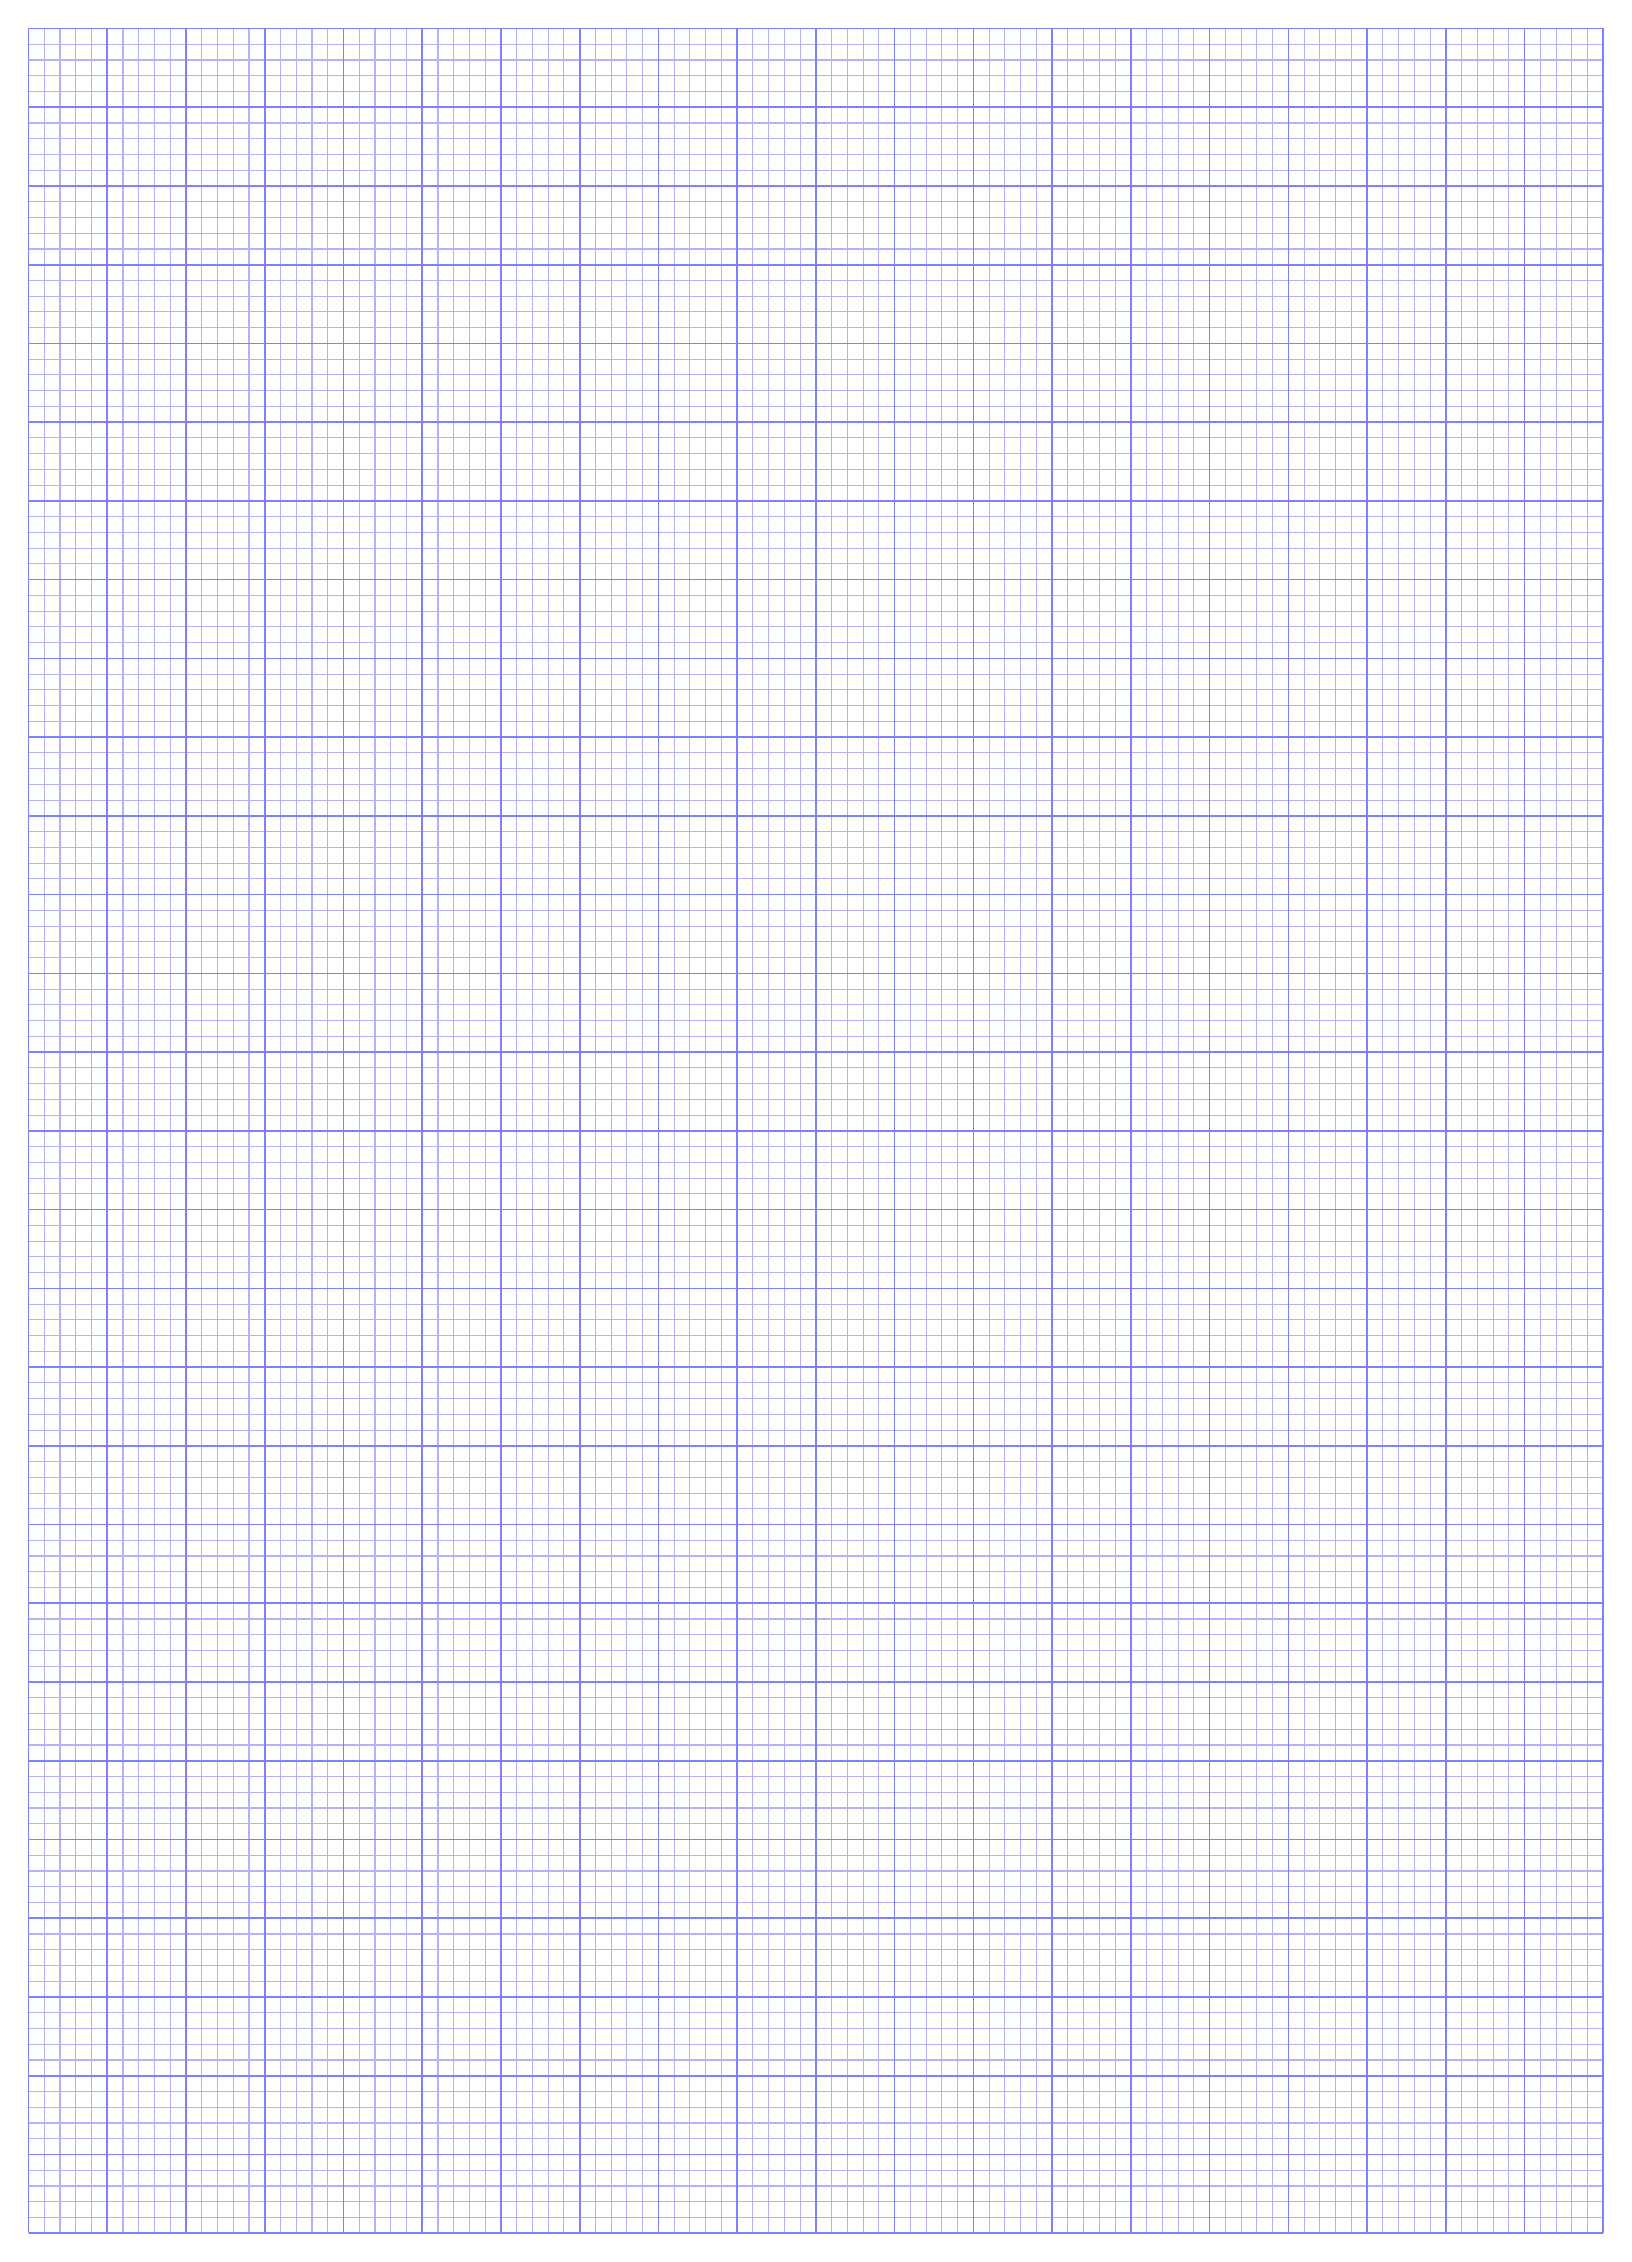
\begin{tikzpicture}
% \draw[blue,very thin](0,0)grid[step=0.5cm](6.5,10);
\draw[line width=.4pt,draw=blue!30] (0,0) grid[step=2mm] (20,28);
\draw[line width=.6pt,draw=blue!50] (0,0) grid[step=1cm] (20,28);
\end{tikzpicture}
